\documentclass[a4paper,10pt]{article}

\usepackage[utf8]{inputenc}
\usepackage{lmodern}
\usepackage{microtype}

\usepackage{graphicx}

\usepackage[english]{babel}
\usepackage[autostyle, english = british]{csquotes}
\MakeOuterQuote{"}

\usepackage[framemethod=tikz]{mdframed}

\def\signed #1{{\leavevmode\unskip\nobreak\hfil\penalty50\hskip2em
  \hbox{}\nobreak\hfil(#1)%
  \parfillskip=0pt \finalhyphendemerits=0 \endgraf}}
\newsavebox\mybox
\newenvironment{aquote}[1]
  {\savebox\mybox{#1}\begin{quote}}
  {\signed{\usebox\mybox}\end{quote}}

\title{Scholarship Classical Studies: Exam Advice}
\author{Alex Elzenaar}

\begin{document}

\maketitle
\begin{abstract}
  This article is a set of advice for candidates sitting the NZ Scholarship Classics exam --- specifically
  on question interpretation and essay writing. No apologies are made for the rambling nature of the exposition!
\end{abstract}

\tableofcontents

\section{The scholarship performance standard (93404)}
\subsection{Outcome Description}
The student will use knowledge of classical studies to demonstrate their ability to think critically about the ideas and values of the classical world. They will communicate their understanding through the use of primary and secondary source evidence in a range of integrated contexts, which may include history, literature, philosophy, architecture and / or art.

\subsection{Performance Descriptors}
\subsubsection{Scholarship}
The student will demonstrate aspects of high level:
\begin{itemize}
  \item analysis and critical thinking
  \item integration, synthesis, and application of highly developed knowledge, skills, and understanding to complex situations
  \item logical development, precision and clarity of ideas.
\end{itemize}

\subsubsection{Outstanding}
In addition to the requirements for Scholarship, the student will also demonstrate, in a sustained manner, aspects of:
\begin{itemize}
  \item perception and insight
  \item sophisticated integration and abstraction
  \item independent reflection and extrapolation
  \item convincing communication.
\end{itemize}

\subsection{Explanatory Notes}
\begin{enumerate}
  \item This standard is derived from the Social Sciences learning area in the New Zealand Curriculum (Learning Media, Ministry of Education, 2007) up to and including Curriculum Level 8, and the Classical Studies Teaching and Learning Guide.
  \item Subject specific definitions:
  \begin{itemize}
    \item Analysis and critical thinking requires methodical examination and interpretation of primary and secondary source
          evidence and an awareness of their limitations.
    \item Integration, synthesis and application of highly developed knowledge, skills and understanding to complex situations
          involve using a range of information and applying understanding of the ideas and values of the classical world to
          explain links and interrelationships.
    \item Perception and insight involves subtlety of understanding, an awareness of subtext, and historical empathy.
    \item Sophisticated integration and abstraction involves the ability to identify and interpret specific elements of a wide
          range of evidence and to formulate a complex perspective of the ideas and values of the classical world.
    \item Independent reflection and extrapolation involves drawing upon a wide range of evidence and, through the selection and
          exploration of relevant elements, challenging the basis of assumptions and perceptions.
    \item Convincing communication requires a coherent and fluent response with a degree of literary flair and originality.
  \end{itemize}
\end{enumerate}

\section{The Exam Layout}
You should expect to write three essays: two on topics of your choice (section A), and one resource based topic (section B). The topics
which you can choose from for section A will probably\footnote{~An up-to-date list can be found in the Assessment Specifications for the
year you are sitting the exam; see the NZQA website.} include:
\begin{itemize}
  \item Alexander the Great
  \item Augustus
  \item Socrates
  \item Virgil's \textit{Aeneid}
  \item The plays of Aristophanes
  \item Athenian vase painting
  \item Roman art and architecture
\end{itemize}

For section B, the topic will be announced in the assessment specifications as it changes from year to year (so you get it in advance); you
will also typically get a choice between focusing on the Greek or the Roman side of your topic. The topics generally are something like:
\begin{itemize}
  \item Religion and the gods
  \item Death and the underworld
  \item Conflict and warfare
  \item Culture and identity
\end{itemize}

\emph{Know what topics you want to write essays on beforehand. Have at least THREE topics that you would be comfortable with for the long-form
      essay section just in case the questions are unfriendly.}

\section{Preparing for the Exam}
There is a reason that I run scholarship classics tutoring as a reading course: the best way to know and understand the material
is to connect with it and immerse yourself in the sources.

Know the sources well, know their strengths and weaknesses, know the main ideas and the sweeping generalisations. Details are nice,
but don't sit down and try to memorise them at the expense of general understanding of the big picture. The latter is worth much
more in scholarship than the former.

Don't just reread the standard commentaries and sources over and over again; go out looking for new material, find stuff to disagree
with, and write down the name of the author. Don't just read plays, read other writer's perspectives on the plays. Find controversy,
work out which side you're on, and try to justify it. You should not avoid material that you disagree with; on the contrary, it is
normally much easier to write on (and shows more independent thinking)!

\section{Interpreting Questions}
The most important thing about scholarship questions (compared to those that appear on the level three examinations) is that they
are not formulaic, and so require you to interpret them. The examiner is not looking for a rote-learned essay, but an ability to
argue a point of view on a matter that may not have an obvious answer.

\subsection{Section A}
The following rather long-winded question appeared on the 2016 scholarship exam.

\begin{mdframed}
  After the battle of Issus, Alexander captured members of the Persian royal family, including Darius’ wife. Quintus~Curtius~Rufus
  praised his treatment of the captives:

  \begin{aquote}{Quintus Curtius Rufus}
    "At this particular time, certainly, his actions were such that he outshone all previous kings in self-control
    and clemency* ... As for Darius’ wife, who was surpassed by none of her generation in beauty, Alexander
    was so far from offering her violence that he took the utmost care to prevent anyone from taking
    advantage of her."
  \end{aquote}
  To what extent were self-control and clemency the hallmarks of Alexander’s treatment of those he
  conquered?

  *\small{\textit{clemency}: mercy}
\end{mdframed}

Scholarship questions from section A usually begin with a quote, and then the question asks you to respond to a related idea or
concept. The quotes used are usually also a hint as to how the examiner wants you to answer the question.

In this case, the examiner is asking about the mercy shown by Alexander the Great to those he captured. They are looking
for two things:
\begin{itemize}
  \item A \emph{point of view} regarding Alexander's treatment of those he conquered (was he relatively merciful?), and
  \item An \emph{intelligent argument} backing that point of view up.
\end{itemize}

In answering this question, you would be expected to define clemency, relate events from Alexander's life (with reference to
both primary and secondary sources), and come to a conclusion (after considering all the possible points of view). In one sense,
it is a rather simple question: you only need to write one argument, and it would be relatively easy to conclude one way or the
other in a balanced way.

A shorter but more complex `personality' question comes from the Roman art section of the 2015 exam:

\begin{mdframed}
  \begin{aquote}{Cornelius C. Vermeule III}
    "The Romans loved portraits of themselves. They embellished their public spaces with statues and
    busts of their emperors ... [and their] coins feature ... precise portraits of famous leaders."
  \end{aquote}
  To what extent were imperial portraits* faithful images of the individuals portrayed? What factors might
  account for divergence from realistic portraiture?

  *\small{`Imperial portraits' include the representation of emperors in statues, sculptural reliefs, cameos, and / or on coins.}
\end{mdframed}

This question has two parts: a `describe' part (where you must draw on your factual knowledge, providing examples of both faithful
and unfaithful portraits) and an `interpret' part (where you must say something intelligent about the reasons behind these examples
and draw an insightful conclusion about Roman society).

The quote here is not as evocative (to me, anyway) as the Alexander quote above --- however, a nice essay could use the phrase `the Romans
loved portraits of themselves' as a springboard to talk about the cultural reasons for propaganda in portraiture (i.e. portraits were the only
way for the outer reaches of the Empire to `see' their emperor), and could form the conclusion around the correctness (or lack thereof)
of the use of the word `precise' by Vermeule. (Interesting point: does the word `precise' here mean \emph{well-executed technically and
artistically}, or \emph{true to life}? Write an essay on this.)

My personal preference is to focus on the `describe' part when choosing a question: it's usually possible to say something intelligent
about anything as long as you have enough examples, so even if you cannot come up with a thread to pull all your examples together
when you're looking at a question then it may be worth choosing it anyway if you have enough basic knowledge.

\begin{center}
  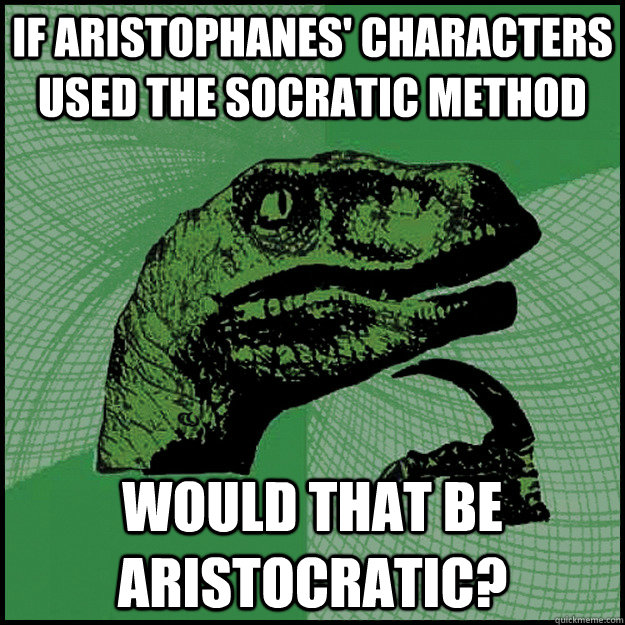
\includegraphics[width=0.3\textwidth]{aris}
\end{center}

The theatre questions are often relatively bare-bones. The following question on Aristophanes comes from the 2015 exam:
\begin{mdframed}
  How valid is it to argue that Aristophanes sees the problems facing Athens as insoluble and, in response,
  uses absurd fantasy as a form of escapism?
\end{mdframed}

Note here the wording `How valid is it to argue...', rather than the alternative `Is it valid to argue...'. This is a good example
of the open-ended nature of scholarship questions. The examiner is not looking for a straight yes/no answer --- they are looking
for a \emph{reasoned and balanced argument}, that looks at all of the sides of the coin and then makes a justified conclusion. If
you can only think of arguments for one side (or can only think of one side to argue), then do not pick that question!

Noticing the lack of a quote here is also a nice segue into a discussion of the role of quotes in theatre essays: the examiners
are not looking for a regurgitation of \textit{Frogs} or \textit{Lysistrata}, but a general discussion of Aristophanes' purpose.
Because of this, you will be talking about the general ideas throughout the text rather than doing a close-reading analysis. Quotes
are nice, but not necessary (and gratuitious quotes make it look like you have no original ideas of your own). A well-chosen
quote of five words that is used within your argument is much better (and shows better fluency) than taking a passage from Aristophanes
and just dropping it into the middle of your prose (even if you introduce it).

To get back to the question itself, the examiner is looking for two things (framed as one question this time):- (1) whether Aristophanes
sees the problems facing Athens as insoluble (debatable, he proposes solutions a few times with only a little sarcasm) and (2) whether
Aristophanes' use of absurd fantasy (\`a~la \textit{Birds} or \textit{Lysistrata}\footnote{~Yes, I would call \textit{Lysistrata} `absurd
fantasy' since it has been argued (conclusively in my mind) that Aristophanes is not actually promoting a classical form of feminism or
equality but is simply presenting this situation as a mark of how absurd the situation has grown: the idea that women could (gasp!) be
competent and full members of society would have been comedic to the conservative and varied audience of the play. Aristophanes intended
his portrayal of the sex strike and seizure of the temples to be absurd, and put forward to the audience the idea that `peace is such a
simple solution that even a woman could think of it!'. Of course, in our (hopefully) more enlightened times the ideas are only comedic in
their tone but not their modern equalist overtones.}) is not only for comedic effect, but for the far less respectable goal of escapism (surely
he would not stoop that low...)!

See how I spun that question? Let's try to spin it the other way:

To get back to the question itself, the examiner is looking for two things (framed as one question this time):- (1) whether Aristophanes
sees the problems facing Athens as insoluble (quite likely, since the only solutions he tries to put forward are over-the-top and obviously
for comedic effect) and (2) whether Aristophanes' use of absurd fantasy (\`a~la \textit{Birds} or \textit{Lysistrata}) is only to provide
escapism and temporary relief from the peaceless and hopeless situation that the Athenians found themselves in, just years before the
dismantling of their democracy!

I hope I have made my point --- there are a myriad of perspectives to every question.

\subsection{Section B}
The questions from Section B, on the other hand, are very formulaic; from 2016, we have:
\begin{mdframed}
  Choose EITHER ancient Greece (Resources A–D) OR ancient Rome (Resources E–H) to answer this
  question. The resources provide evidence about death and the afterlife in the classical world.

  Discuss at least THREE of the resources and the insight they give into Greek or Roman beliefs and
  practices linked to death and the afterlife.

  Your response should focus on analysis of the source material provided, but you should also draw on
  your wider knowledge of the classical world.
\end{mdframed}
I do not think much commentary here is necessary; you know what topic(s) will be available beforehand,
so you need only really prepare for one question.

\section{Writing Essays}
\begin{center}
  
\includegraphics[width=0.5\textwidth]{essay}
\end{center}
So you've chosen your question, and want to write your essay.

\subsection{The Introduction}
I tend to write essays as a flow-of-consciousness, and so when I write my introductions I usually have no idea what
my conclusion will look like. In fact, when I sat the Scholarship paper myself, I changed my final answer to the question
halfway through! As such, I tend to think that a good paragraph introduces the subject, summarises the question, gives your
interpretation of the question, roughly outlines the vague shape of your argument, and then gets out of the way without
giving much hint of what your conclusion will be.

A better justification for this kind of introduction is that you want your marker to keep reading: if you give the
punchline away at the start, then there is no mystique around your argument and nothing to set your paper apart
from the last sixty boring ones that they have read.

An extremely bare-bones example of an introduction for a literature which meets those criteria is as follows (from an essay on Catullus' Poem LXIV):
\begin{mdframed}
  Gaius Valerius Catullus was a Roman neolitic poet active in the first century BCE. Over 100 of Catullus' poems
  survive in almost complete form including the avant-garde Poem 64, an epyllion which contrasts the expectations
  of society with respect to epic heroism with themes of love and marriage, and overall it seems that Catullus was
  trying to present love as the more powerful force of the two.
\end{mdframed}

I do feel, in retrospect, that this introduction is a bit too light for a serious essay; its purpose was to immediately lead
into a close analysis of the text and as such contains the bare minimum of niceities. I think that a better version of this
would have a few sentences giving a couple of examples of the contrasts mentioned, and a sentence summarising the plot
and point\footnote{~Although, to be honest, the `point' of poem 64 was the focus of the entire essay and so summarising it
here would go against my most fundamental guideline: don't rewrite your conclusion to serve as an introduction!} of poem 64.

The following introduction to an essay on Alexander the Great is probably more what I would be expecting for scholarship:
\begin{mdframed}
  Alexander the Great was born in 356 BC to Phillip II, king of Macedonia, and Olympias of Epirus; he grew to rule
  one of the greatest empires in Western history, stretching from the Balkans in the west to the Indus River in the
  east. Despite his importance to classical history, modern historians have limited reliable information about Alexander's
  life. This is due to the lack of extant primary sources, forcing us to rely on later writers like Plutarch, Arrian, and
  Diodorus, and to the inherent bias present in all sources due to Alexander's hero-or-villain persona, and the actions
  which he carried out for propaganda purposes in order to win the support of his men and of the people living in the
  countries he conquored. Arrian wrote that Alexander was "the most variously written about" of all leaders in history,
  and the noted modern writer Brian Bosworth shared a similar sentiment, writing that in the 1980s, a new book about
  Alexander was coming out every year. These two statements show just how many different  and often contradictory ideas
  it is possible to have about Alexander, and therefore how careful we have to be in analysing source material and attempting
  to reconstruct his motivations and actions.

  Many myths surrounded Alexander's birth and early life. His parents both believed that they were descended from heroes
  and deities, including Heracles, Perseus, and Achilles, and the Roman writer Plutarch writes about rumours that Alexander
  himself was the son of Zeus, after his mother was seen with a serpent (a form often taken by Zeus in Greek myth) in her bed.
  Alexander was brought up reading Homer, including the Iliad – the epic poem telling the story of the Trojan War, which a
  copy of which he kept with him all through his life. With such a childhood, it is not entirely surprising that, as a ruler,
  religious beliefs were an important part of his image; in fact, Alexander was a master of religious propaganda.
\end{mdframed}

This introduction is quite nice for an Alexander essay: it summarises his life in one sentence, gives a glimpse of the problems
with the source material, introduces the topic of the essay (the use of religious propaganda by Alexander) in its proper historical
context, and has a nice catchy punchline. Notice, though, that it doesn't have mounds of verbiage (and gives only a few hints as to
how I will go about justifying my final statement).

I do tend to be a little loose with the traditional essay structure (introduction, self-contained paragraphs, conclusion); confidence
and fluency are important skills for the professional essay writer. Be creative with the paragraph structure, don't be afraid to have
a short introduction and get straight into the meat, and remember not to summarise your argument before it begins.

\subsection{A Typical Paragraph}
This out-of-context paragraph is taken from an essay on Plautus' play \textit{The Swaggering Soldier}:
\begin{mdframed}
  The scene is out-of-place, separating the two halves of the action of the play and not really furthering the storyline
  in any way; Watling calls the scene "unnecessary" in his introduction to the translated version (p. 149). The obvious
  answer is that Plautus was trying to make a point and to put forward his views on an issue. Interestingly, many of the
  views put forward are counter to the general values of Roman society. One of the fundamental tenets of Roman society was
  the duty of the citizen to his family and his country, and this included the duties of men to marry, start a family, and
  offer hospitality to guests. I am not so sure that Plautus would seriously present the view that such a fundamental principle
  was wrong, especially given the success that the play apparently enjoyed at the time.

  Another explanation, and one which is probably more likely, is that these lines are a bit of tongue-in-cheek humour similar
  to modern American sitcom humour, expressing the sentiment that women and family only cause trouble for men with their constant
  nagging and requests for money, in an attempt to elicit laughter --- apparently this type of comedy has endured throughout the
  past millenia, probably since it pokes fun at such a fundamental part of Western society.
\end{mdframed}

I would not claim it to be the best paragraph I have ever written, but it is illustrative of a number of points which I wish
to make.

Firstly, as I alluded to above, I am not a fan of taking long quotes from primary or secondary sources and sticking them into
the essay vertabim; my preferred style is to paraphrase the quote, and then pick out a few nice words and directly quote those.
The Alexander introduction above has a few more examples, but I suppose the most important thing is to remember to only recall
a quote if it is absolutely necessary; that is, you want to discuss the idea in the quote at some length. Pulling quotes in just
because you want to fill an imagined quota does not look great.

Secondly, notice the lack of a rigid structure. The point of a scholarship essay (or any essay, really) is to make a point about
the bigger picture, and so the paragraphs should flow into each other and work to bring the reader into your conclusion. On
the other hand, write in the way that is most comfortable for you. If you find you work best when you have a structure in mind,
then by all means write that way! Just make sure that it all fits together as a cohesive whole.

Note also the way that the essay topic plays a central role. \emph{You are not writing an essay on Alexander the Great, on Socrates,
on art; you are writing a response to a topic related to them!} In other words, always explain how the quotes you give or events you
relate are not only relevant but \emph{irreplacable} in efforts to understand the topic. Give multiple explanations and discuss which
one you feel is most likely, and then link it back to the big overall point that you are trying to make.

Link everything back to the culture of the time (whether it is Hellenistic, Alexandrian, Augustan, Constantinian, or otherwise), and
try to describe why the topic that you are writing about is relevant to a proper historical or literary understanding of the time
period.

Overall, though, remember that it is the content that you write and the ideas that you put forward that matter; presentation is just
a bonus. (Not that you should neglect the presentation, that is --- it should be a consideration, just don't let your argument suffer
for the sake of making it sound better.)

\subsection{Dealing with Sources}
\begin{aquote}{2016 Examiner's Report}
  All questions allowed candidates to produce answers of scholarship standard and --- at the top end --- critical commentaries on the
  source documents were notably sophisticated and insightful. Candidates who were awarded Scholarship with Outstanding Performance
  commonly... integrated relevant primary and secondary source evidence into their response.
\end{aquote}
An important part of scholarship is knowledge of a wide variety of both primary and secondary sources. There is no nice way to say this:
\begin{center}
  
\includegraphics[width=\textwidth]{sources}
\end{center}

You should have a variety of sources that you can pull from during the exam, knowing both their content and their strengths and
weaknesses. For some topics, like Alexander the Great, we do not have any extant primary sources and so the examiners are looking for
an understanding of the problems associated with this. Challenge the sources of evidence for bias and propaganda.

It goes without saying that any statement you make in an essay should be backed up by primary or secondary sources; the markers in
an exam will be less strict about this (especially as the material is quite standard), but you will be penalised if you do not refer
to any primary sources!

Knowledge of secondary sources is also very important; not only to quote to support arguments, but to pull in to compare and contrast
with your own argument.

\subsection{The Resource-based Section}
The main advice that I have for the resource-based section is to focus on the resources that they give you, rather than your own
background knowledge. They won't give you anything too nasty; pick an angle that the resources suggest, and then write one paragraph
per resource to back up your angle. Don't overthink this section.

\section{Per-topic Advice}
I am not so egotistical that I will attempt to give advice on topics that I know nothing about; I may add subsections here as and
when I have time to go and learn the material.

\subsection{Alexander the Great}
\begin{center}
  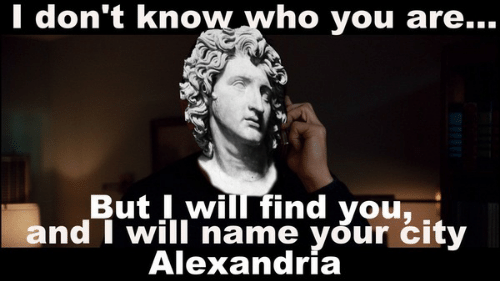
\includegraphics[width=0.3\textwidth]{alexander}
\end{center}
There are two main facets to Alexander: strategy and personality. I have always personally found a personality essay much
easier to write (it is less difficult to find an new and interesting point to make).

The important strands of Alexander's personality include:
\begin{itemize}
  \item His childhood and upbringing.
  \item His ego and ambition politically and militarily.
  \item His religious beliefs, and his views on his own deification.
  \item More generally, his use of propaganda.
  \item His attitude towards the peoples that he conquered.
\end{itemize}

Strategically, some areas of interest include:
\begin{itemize}
  \item The siege at Tyre.
  \item The other battles with Darius' armies.
  \item The founding of Alexandria.
  \item His drive further eastwards.
  \item The `mutinies'.
\end{itemize}

Have a general understanding of all the topics, and the big picture; but pick a few and know them well.

\subsection{Roman Art and Architecture}
Use this as an excuse to learn Roman history from Augustus to Constantine. Some good pieces to focus on include
\begin{itemize}
  \item Idealised images of Augustus (e.g. Prima Porta)
  \item \textit{Togatus Barberini} (?)
  \item The bust of Commodus
  \item The arch of Septimius
  \item Busts of Philip the Arab
  \item The arch of Constantine
\end{itemize}
but the best way to approach this topic is to use the art to talk about Roman politics and society (not the other way around).

Pick up a good long book with lots of pictures that covers the whole Roman age, and read bits of it at a time to get a big-picture overview.

\subsection{Aristophanes}
Know the history of the era that Aristophanes was writing in. If you are writing about war and conflict, make sure you
read Thucydides (or at least Hanson) before you try to tackle \textit{Peace}, \textit{The Archarnians}, \textit{Lysistrata},
or any of Aristophanes' other war-related works. If your focus is on politics, revise Socrates and Plato before reading \textit{The Clouds}
or \textit{The Birds}. Find someone who knows the era, and get them to help you to focus your attention.

Secondary sources on Aristophanes (especially the introductions and notes in the Penguin editions) are your friend.

\end{document}
